\documentclass[11pt]{article}
\usepackage[utf8]{inputenc}
\usepackage[T1]{fontenc}
\usepackage[a4paper]{geometry}
\usepackage{minted}
\usepackage{multirow}
\usepackage{enumerate}
\usepackage{tikz}

%% for listings..
\definecolor{mintedBg}{rgb}{0.95, 0.95, 0.95}
\definecolor{blockBg}{rgb}{0.6, 0.6, 0.95}
\newminted{perl}{linenos, bgcolor=mintedBg, fontsize=\footnotesize}
\newminted{r}{linenos, bgcolor=mintedBg, fontsize=\footnotesize}
\newminted{console}{linenos, bgcolor=mintedBg, fontsize=\footnotesize}

\setcounter{page}{2}

\begin{document}

This exam contains a total of 8 sections. The majority of these sections have
some choice in the questions that you answer. Please read the instructions
below each section head. A total of 100 marks will be considered as full marks.

The number of marks available from each section is indicated in the section
headings. Note that it is possible to select questions that total more than
that mark; however, you will not be able to get more marks from a given
section by answering more questions. If you find that your answer to a given
question is no good and you wish to change your selection, then cross out the
old one to indicate which one you do not wish to be marked for.

Feel free to illustrate your answers wherever you feel appropriate; but do
remember to include labels so that I can decipher your figures. Do not include
a picture without some descriptive text. Two of the questions will need to be
filled in on a supplementary sheet. Do not forget to hand this in with your
other answers.

Marks have been assigned on the assumption of a four hour exam; that is one mark
corresponds to 2.4 minutes. For some of the questions that may mean mostly
writing, but for others (esp. code and manual snippets) that time may be taken up by
reading the details of the question, and the answer itself may be very
short.

\section{Bioinformatics in General (12 points)}
Answer all questions in this section.
\begin{enumerate}
\item What is bioinformatics and why is it becoming an essential topic for
  biologists?\\
  Note that the there is no single correct answer to this question, and that
  you will not be judged on what you argue, but on how reasonable and informed
  your argument is.
  
  In your answer you may wish to consider the following:
  \begin{itemize}
  \item your opinion of what bioinformatics is
  \item the technologies or skills that are used within the field
  \item the impact of technological process on biological experiments
  \end{itemize}
  (6 points)

\item A large part of bioinformatics deals with the analysis of sequences.
  \begin{itemize}
  \item Why is there such an emphasis of the analysis of sequences within
    bioinformatics? (Any reasonable answer will be accepted).\\
  \item What property of sequence data distinguishes it from other types of
    biochemical data?
  \item Describe an example of DNA sequence analysis that does not involve the
    alignment of sequences.\\
  \item What's the general relationship between sequence alignment and
    sequence comparison?\\
  \end{itemize}
  (6 points)
\end{enumerate}


\section{Molecular Biology \& the Central Dogma (20 points)}
Answer questions giving a total of 20 points for this section.
  
\begin{enumerate}
\item Describe how proteins are encoded in genomic sequences and how this
  information is transmitted and utilised in protein synthesis. Include in
  your answer a comparison between pro- and eukaryotic genomes. Remember to
  include details of:
  \begin{itemize}
  \item Gene structure
  \item How the structure relates to the regulation of the gene
  \item The encoding of amino acids in nucleic acid sequence
  \item Protein synthesis
  \item The cellular locations of the processes
  \end{itemize}
(8 points)

\item The central dogma refers to how information encoding protein sequences
  is copied and utlised to produce functional molecules. Describe three exceptions
  to the central dogma.\\
(4 points)

\item Given a genetic code:\\
  \begin{minipage}{0.6\textwidth}
  {\tiny
    %% this requires 
%% usepackage{multirow}
%% usepackage{tabularx}

\renewcommand{\arraystretch}{1.25}
\begin{tabular}{ |l| l l|l l| l l|l l|l| }
  \hline
  \multirow{2}{2em}{1st base} &
  \multicolumn{8}{|c|}{2nd base} &
  \multirow{2}{2em}{3rd base} \\
  \cline{2-9}
  &
  \multicolumn{2}{|c|}{U} &
  \multicolumn{2}{|c|}{C} &
  \multicolumn{2}{|c|}{A} &
  \multicolumn{2}{|c|}{G} & \\
  \hline
  \multirow{4}{2em}{U} & 
  UUU & \multirow{2}{4em}{\tiny (Phe/F)} &
  UCU & \multirow{4}{4em}{\tiny (Ser/S)} &
  UAU & \multirow{2}{4em}{\tiny (Tyr/Y)} &
  UGU & \multirow{2}{4em}{\tiny (Cys/C)} & U \\
  & UUC & & UCC & & UAC & & UGC & & C \\ \cline{2-3} \cline{6-9}
  & UUA & \multirow{6}{4em}{\tiny (Leu/L)} 
  & UCA & & UUA & Stop & UGA & (Stop) & A \\ \cline{8-9}
  & UUG & & UCG & & UAG & Stop & UGG & \tiny (Trp/W) & G \\ \cline{4-9} 
  \cline{1-1}
  \multirow{4}{2em}{C}
  & CUU & & CCU & \multirow{4}{4em}{(Pro/P)} & CAU & \multirow{2}{4em}{(His/H)} & CGU & \multirow{4}{4em}{(Arg/R)} & U \\
  & CUC & & CCC & & CAC & & CGC & & C \\ \cline{6-7}
  & CUA & & CCA & & CAA & \multirow{2}{4em}{Gln/Q} & CGA & & A \\
  & CUG & & CCG & & CAG & & CGG & & G \\ \cline{1-9}
  \multirow{4}{2em}{A}
  & AUU & \multirow{3}{4em}{(Ile/I)} & ACU & \multirow{4}{4em}{(Thr/T)} & AAU 
  & \multirow{2}{4em}{(Asn/N)} & AGU & \multirow{2}{4em}{(Ser/S)} & U \\
  & AUC & & ACC & & AAC & & AGC & & C \\ \cline{6-9}
  & AUA & & ACA & & AAA & \multirow{2}{4em}{(Lys/K)} & AGA & \multirow{2}{4em}{(Arg/R)} & A \\
  \cline{2-3}
  & AUG & (Met/M) & ACG & & AAG & & AGG & & G \\ \cline{1-9}
  \multirow{4}{4em}{G}
  & GUU & \multirow{4}{4em}{(Val/V)} & GCU & \multirow{4}{4em}{(Ala/A)} 
  & GAU & \multirow{2}{4em}{(Asp/D)} & GGU & \multirow{4}{4em}{(Gly/G)} & U \\
  & GUC & & GCC & & GAC & & GGC & & C \\ \cline{6-7}
  & GUA & & GCA & & GAA & \multirow{2}{4em}{(Glu/E)} & GGA & & A \\
  & GUG & & GCG & & GAG & & GGG & & G \\ \hline
\end{tabular}

  }
  \end{minipage}

  Given the following genomic sequence:\\
  \verb|GCGATGGGCGGTGGGGTG|\\
  determine all possible translations.\\
  (4 points)

\item What is an open reading frame (ORF)? Describe how they can be used to identify
  genes in non-annotated genome sequences? Why is this easier in prokaryotic
  than eukaryotic species?\\
  (4 points)

\item Describe three different kinds of mutations that can arise in DNA
  sequences and how the consequences of mutations vary depending on their location.\\
  (4 points)

\item DNA sequences are generally double stranded with two complementary
  strands forming a double helix.
  \begin{itemize}
  \item What is meant by two nucleic acid strands being complementary?
  \item What effect does double-strandedness have on the structure of DNA? Why
    does this matter?
  \end{itemize}
(4 points)

%% \item How do the monomers of nucleic acids differ from those of proteins? How
%%   does this relate to their function?\\
%% (4 points)

\item What is a codon? How long is it and why? Explain how this leads to the
  degeneracy of the genetic code.\\
(4 points)
\end{enumerate}

\section{Biological databases \& formats (8 points)}
Answer questions giving a total of 8 points for this section.
\begin{enumerate}
\item Describe the typical structure of a web-facing databases. Comment on the
  different types of users and on how they use the database differently.\\
  (4 points)

\item Given a novel nucleic acid sequence obtained from a non-model organism
  describe  the steps you can take to
  determine the likely function of the sequence. Include seperate descriptions
  for:
  \begin{itemize}
  \item A transcribed mRNA sequence
  \item A genomic sequence
  \end{itemize}
  The steps taken for the analysis depend to some extent of the length of the
  sequence you start with; for this question you may assume a sequence length
  of around a 1000 nucleotides.\\
  (8 points)

\item The SAM format is used to describe the alignments of large numbers of
  sequences to a common reference sequence (typically a genome sequence). Each
  alignment is described by a single line of tab delimited text. The second
  field of this description is a FLAG that uses a single number to encode
  speficic combinations of 12 flags that indicate individual
  properties of problems of the sequences or alignments as indicated by the
  following table:

  {\small
  \begin{tabular}{rrl}
    Bit & Value & Description\\
    \hline
    1 & 1 & template having multiple segments in sequence \\
    2 & 2 & each segment properly aligned according to the aligner\\
    3 & 4 & segment unmapped\\
    4 & 8 & next segment in the template unmapped\\
    5 & 16 & SEQ begin reverse complemented\\
    6 & 32 & SEQ of the next segment in the template being reverse complemented\\
    7 & 64 & the first segment in the template\\
    8 & 128 & the last segment in the template\\
    9 & 256 & secondary alignment\\
    10 & 512 & not passing filters, such as platform quality controls\\
    11 & 1024 & PCR or optical duplicate\\
    12 & 2048 & supplementary alignment\\
  \end{tabular}
  }

  Each of the above numbers is an exact power of 2 which means that it is
  encoded in binary by a single 1 in the appropriate position. A single
  number can thus hold any combination of the given flags and
  a given flag value can be checked by a bitwise AND operation. For example,
  if a given sequence failed to pass filters, and has been reverse
  complemented we set the 10th (512) and 5th (16) bits to 1 giving us 528 (512 +
  16).\\
  Describe the meanings of the following FLAG values: 0, 16, 272, 512.\\
  (4 points)
\end{enumerate}


\section{Pairwise alignment (20 points)}
Answer questions giving a total of 20 points for this section.
\begin{enumerate}
\item For the two sequences: \verb|5' ATTATGCA 3'| and \verb|5' TTAATCA 3'| :
  \begin{enumerate}
    \item Provide at least two reasonable alignments.
    \item Describe how you can score the alignments using sets of penalties
      or scores.
    \item Score the alignments using at least two different sets of
      penalties. 
    \item Which of your alignments do you think is most reasonable and why? 
    \item Are your alignments global or local?
  \end{enumerate}
  (10 points)

\item Why do we often use a different penalty for gap insertion and gap
  extension? Provide an example alignment with your question.\\
  (4 points)

\item Fill in the first three rows and columns of the following
  alignment table for a global alignment (Needleman-Wunsch). Include
  both scores and back-track information. (Use the supplementary sheet.)
  \begin{figure}[H]
    \begin{tikzpicture}[scale=0.6]
      \input{2016_nm.tikz}
    \end{tikzpicture}
  \end{figure}
  (6 points)

\item What does the following figure contain?
  Obtain all optimal alignments from it:
  \begin{figure}[H]
    \begin{tikzpicture}[scale=0.6]
      \input{sm_2016_a.tikz}
    \end{tikzpicture}
  \end{figure}
  \begin{enumerate}
  \item Draw the process directly on the table on the supplementary sheet.
  \item What kind of alignment(s) did you obtain?
  \end{enumerate}
  (4 points)

%% \item What do we mean by an optimal alignment?\\
%%   (2 points)

%% \item How would you modify the Needleman-Wunsch (global alignment) to
%%   obtain a local alignment (Smith-Waterman)?\\
%%   (4 points)

\item Amino Acid substitution matrices:
  \begin{enumerate}
  \item What are substitution matrices and how do we use them when aligning
    sequences?
%    (2 points)
  \item Describe at least two ways in which you can derive an amino acid
    substitution matrix?
%    (4 points)
  \item On what basis could you define a nucleotide substitution matrix for
    aligning DNA sequences?
%    (2 points)
  \item The following is an example of an amino acid substitution table.
    \begin{figure}[H]
      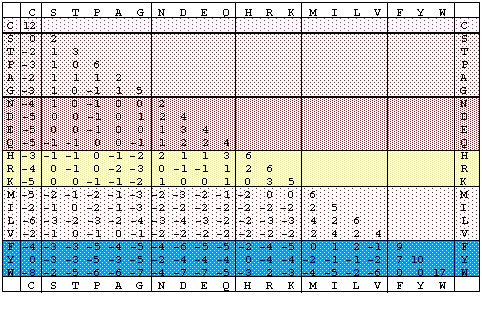
\includegraphics[width=0.7\textwidth]{images/dayhoff_256}
    \end{figure}
    What do the numbers in the matrix indicate?
%  (2 points)
  \end{enumerate}
(10 points)
\end{enumerate}

\section{Multiple sequence alignment (10 points)}
Answer questions giving a total of 10 points for this section.
\begin{enumerate}
\item What are homologues, orthologues and paralogues? Describe how they arise
  during evolution.\\
  (4 points)
\item Why is it useful to align multiple sequences to each other? Give several
  examples where a multiple sequence alignments are used.\\
  (4 points)
\item What are heuristic methods? Why do we use them instead of dynamic
  programming to perform multiple sequence alignment?\\
  (2 points)
\item The Clustal program makes use of a guide tree to perfrom multiple
  sequence alignment. What does this tree represent and how does Clustal
  create this tree?\\
  (6 points)
  
\end{enumerate}

\section{Perl (10 points)}
Answer questions giving a total of 10 points for this section.
\begin{enumerate}
\item In Perl what do the following symbols denote: \verb|$ @ %| ? Give
  examples of how they are used in perl code.\\
(4 points)

\item The following is the code for a small stupid script call \texttt{add.pl}?

  \begin{perlcode}
  #!/usr/bin/perl -w
    
  $a = $ARGV[0];
  $b = $ARGV[1];

  print "$a + $b = ", $a + $b, "\n";
    
  \end{perlcode}

  Describe what happens if you try to run the script using the following
  commands:\\
  \begin{consolecode}
 > perl add.pl 10 5
 > perl add.pl hello world
 > perl all.pl
  \end{consolecode}
  (4 points)
\item What does the following code print?

  \begin{perlcode}
  #!/usr/bin/perl -w

  @a = (0,1);
  for($i = 2; $i < 10; $i++){
    $a[$i] = $a[$i-2] + $a[$i-1];
  }
  
  for $v(@a){
    print $v, ", ";
  }
  print "\n";
\end{perlcode}
(4 points)

\item The following is the manual page for the \texttt{join()} function:\\
  \begin{consolecode}
join EXPR,LIST
  Joins the separate strings of LIST into a single string with
  fields separated by the value of EXPR, and returns that new
  string.
  Example:
  
  $rec = join(':',
              $login,$passwd,$uid,$gid,$gcos,$home,$shell);
  
  Beware that unlike "split", "join" doesn't take a pattern
  as its first argument.  Compare "split".
  \end{consolecode}

  What will the following print:

  \begin{perlcode}
    @words = ("hello", "world");
    print join(' ', @words), "\n";
  \end{perlcode}
(4 points)  
\end{enumerate}

\section{Finding homologous sequences (10 points)}
Answer questions giving a total of 10 points for this section.
\begin{enumerate}
%% \item Describe the relationship between pairwise sequence alignment and
%%   searching a database of sequences for homologous sequences.\\
%%   (2 points)

\item Give a brief description of the Blast algorithm, describing how it is
  applied when searching a protein sequence against protein sequence
  database. Make sure to explain what High-scoring Segment Pairs are and how these
  relate to the amino acid substitution matrix.\\
(6 points)


%% \item You have searched a database for homologous sequences and have obtained
%%   the following results:
%% \begin{figure}[H]
%%   \begin{tikzpicture}[scale=0.5]
        \draw [-, rounded corners, dashed] (1.7,4.9) -- (1.7,5.1) -- (10,5.1)
        -- (10.25, 5.35) -- (10.5,5.1) -- (21,5.1) -- (21,4.9);
        \node [above, scale=0.6] at (10.25,5.25) {Database sequences};
        \draw [-] (1.5,4.3) -- (1.5, 1) node [midway, above, rotate=90,
          scale=0.5] {query};
        \draw [-] (1.7,4.5) -- (4,4.5) node [midway, above, 
          scale=0.5] {db 1};
        \draw [-] (4.2,4.5) -- (7.5,4.5) node [midway, above,
          scale=0.5] {db 2};
        \draw [-] (7.7,4.5) -- (10.3,4.5) node [midway, above,
          scale=0.5] {db 3};
        \draw [-] (10.5,4.5) -- (12.3,4.5) node [midway, above,
          scale=0.5] {db 4};
        \draw [-] (12.5,4.5) -- (15.3,4.5) node [midway, above,
          scale=0.5] {db 5};
        \draw [-] (15.5,4.5) -- (16.5,4.5) node [midway, above,
          scale=0.5] {db 6};
        \draw [-] (16.7,4.5) -- (18.5,4.5) node [midway, above,
          scale=0.5] {db 7};
        \draw [-, dotted] (18.7,4.5) -- (21,4.5);

        \draw [-, line width=1.2] (5,3.8) -- (5.4,3.4);
        \draw [-, line width=0.7] (8,3.8) -- (8.4,3.4);
        \draw [-, line width=0.4] (14.3,3.8) -- (14.7,3.4);
        \draw [-, line width=0.5] (2,2) -- (3,1);

\end{tikzpicture}

%% \end{figure}
%% {\small(db 1, db 2, etc..., refer to individual sequences within the database, the
%% thickness of the diagonal lines refer to local alignment scores)}\\
%% What can you infer from these alignments? How does the choice of database
%% affect the inferences that you can make?\\
%% (4 points)

%% \item Give three different types of nucleic acid sequences (from eukaryotes)
%%   classified by their relationship to genes. How does the type of sequence
%%   used as a query affect the choice of database when searching for homologous sequences?\\
%% (4 points)

%% \item Write down a lookup table (index) for the following sequence:
%% \begin{verbatim}
%% TPATGGANWT
%% \end{verbatim}
%%  (2 points)




%% \item The following is a screenshot of the output from an NCBI blast
%%   search. What do the different columns indicate (consider the total scores
%%   and max scores as a single score for the sake of simplicity). Which of these
%%   scores is usually the most important and why? In your answer refer to how
%%   pairwise sequence alignment is performed. 
%%   \begin{figure}[H]
%%     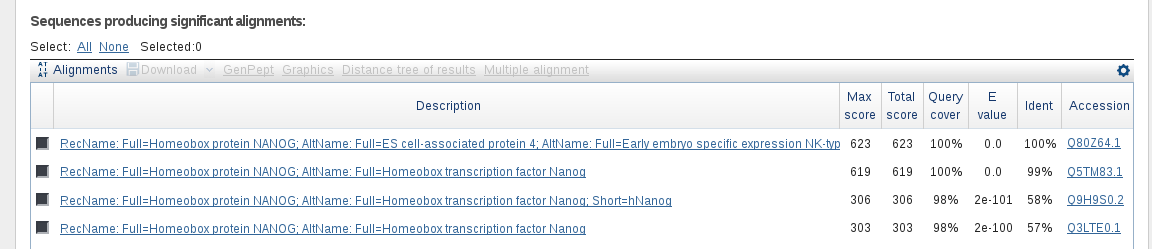
\includegraphics[width=\textwidth]{images/blast_result_list_top}
%%   \end{figure}
%%   (4 points)
  
\item The following is part (very simplified) of the output of \texttt{blastn -help}.\\
  \begin{consolecode}
lmj:[R]> blastn -help 
USAGE                                                                                                                                                 
  blastn [-h] [-help] [-import_search_strategy filename]                                                                                              
    [-db database_name] [-query input_file]                                                                            
    [-out output_file] [-evalue evalue] [-strand strand]
    [-gapopen open_penalty] [-gapextend extend_penalty]                                                                                               
    [-max_hsps int_value] [-num_threads int_value] [-remote]
    [-version]

DESCRIPTION
   Nucleotide-Nucleotide BLAST 2.4.0+

OPTIONAL ARGUMENTS
 -help
   Print USAGE, DESCRIPTION and ARGUMENTS; ignore all other parameters
 -version
   Print version number;  ignore other arguments

 *** Input query options
 -query <File_In>
   Input file name
   Default = `-'
 -strand <String, `both', `minus', `plus'>
   Query strand(s) to search against database/subject
   Default = `both'

 *** General search options
 -task <String, Permissible values: 'blastn' 'blastn-short' 
           'dc-megablast' 'megablast' 'rmblastn' >
   Task to execute
   Default = `megablast'
 -db <String>
   BLAST database name
    * Incompatible with:  subject, subject_loc
 -out <File_Out>
   Output file name
   Default = `-'
 -evalue <Real>
   Expectation value (E) threshold for saving hits 
   Default = `10'
 -num_threads <Integer, >=1>
   Number of threads (CPUs) to use in the BLAST search
   Default = `1'
  \end{consolecode}

  \begin{enumerate}
  \item 
    Write a command that that will use blastn to search a database called
    \texttt{genome\_db} for matches to sequences in the file \texttt{q\_seq.fa}.\\
    You may assume that the files containing the database are present in the
    current working directory.
  \item How might you modify this command if you were searching a database of
    RNA sequences with an mRNA sequence?
  \item How can you make this command run faster?
  \end{enumerate}
  (6 points)


\item There are 5 basic types of blast. Explain what these variants are and
  why they exist. You do not need to give the correct names, though you do
  need to explain the differences in what the programs do.\\
  (6 points)

\item How would you identify an alignment between sequence 1 (\verb|FLWRTWS|) 
  and 2 (\verb|SWKTWT|) from the following table:
\begin{figure}[H]
  \begin{minipage}[t]{0.5\textwidth}
  {\small
    \setlength{\tabcolsep}{0.5em}
    \begin{tabular}[t]{l|ll|l}
      AA & S2 & S1 & S1-S2 \\
      \hline
      S & 1 & 7 & 6\\
      W & 2 & 3,6 & 1,4\\
      K & 3 & & \\
      T & 4 & 5 & 1\\
      W & 5 & 3,6 & -2,1\\
      T & 6 & 5 & -1\\
    \end{tabular}
  }
\end{minipage} 
\begin{minipage}[t]{0.5\textwidth}
  {\small
  Where, \texttt{AA} gives the amino acid residues in sequence 2 located at
  the positions indicated by column \texttt{S2}. Column \texttt{S1} gives
  the lookup table for sequence one. Column \texttt{S1-S2} gives the
  difference between values in \texttt{S1} and \texttt{s2}.
  }
\end{minipage}
  

\end{figure}
{\small Hints: It may help you to plot column \texttt{S1} vs
  \texttt{S2}.
}\\
(4 points)

\item The following is a screenshot of the output from an NCBI blast
  search. What do the different columns indicate (consider the total scores
  and max scores as a single score for the sake of simplicity). Which of these
  columns is usually the most important and why?
  \begin{figure}[H]
    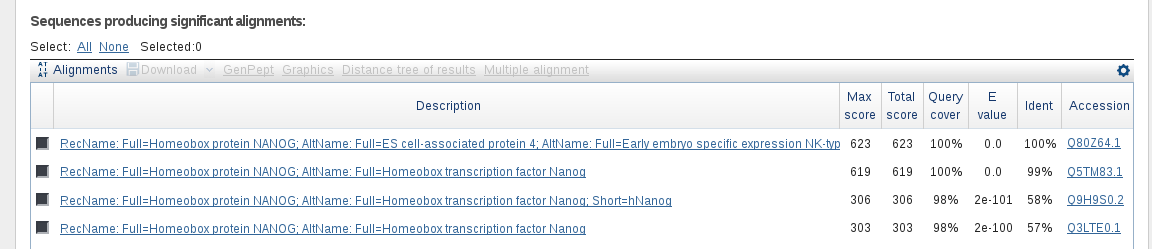
\includegraphics[width=1.2\textwidth]{images/blast_result_list_top}
  \end{figure}
  (4 points)

\end{enumerate}


\section{Numbers, big data and R (10 points)}
Answer questions giving a total of 10 points for this section.
\begin{enumerate}
\item Describe the three most commonly used average values.\\
  (3 points)

\item The following figure shows the distributions of two sets of values \texttt{A}
  and \texttt{B}.
  \begin{figure}[H]
    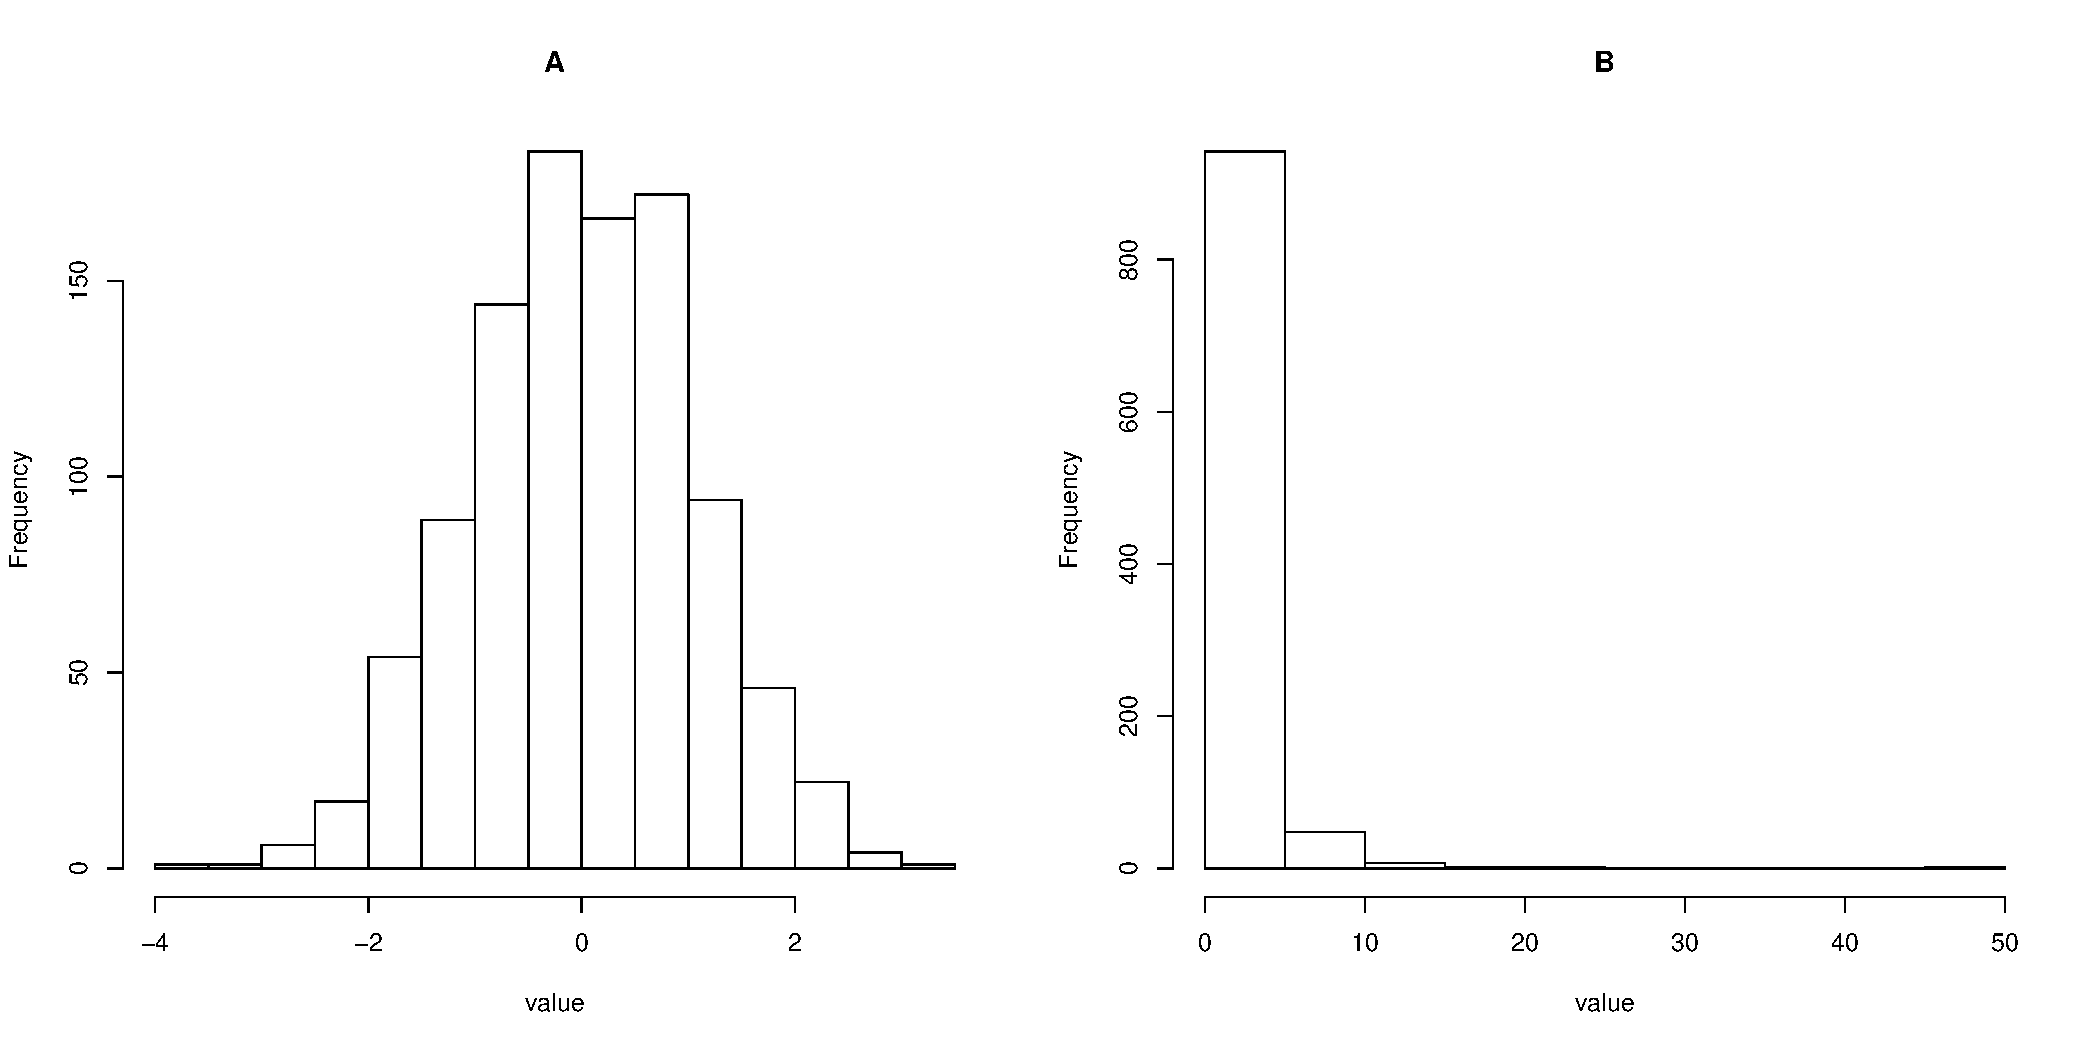
\includegraphics[width=0.8\textwidth]{R/log_norm.pdf}
  \end{figure}
  What type of distribution do you think the values of \texttt{A} follow? What are your
  reasons for thinking this? Estimate the values for the mean, median and mode
  averages for \texttt{A}.\\
  Suggest a distribution for \texttt{B}. Would it be reasonable to calculate
  average values for \texttt{B}? How would you transform the values of
  \texttt{B} before additional analyses?\\
  (6 points)

\item The following plot shows the distribution of a sampling statistic ($X$)
  derived from randomised values that correspond to what would be observed
  under the null hypothesis. 
  \begin{figure}[H]
    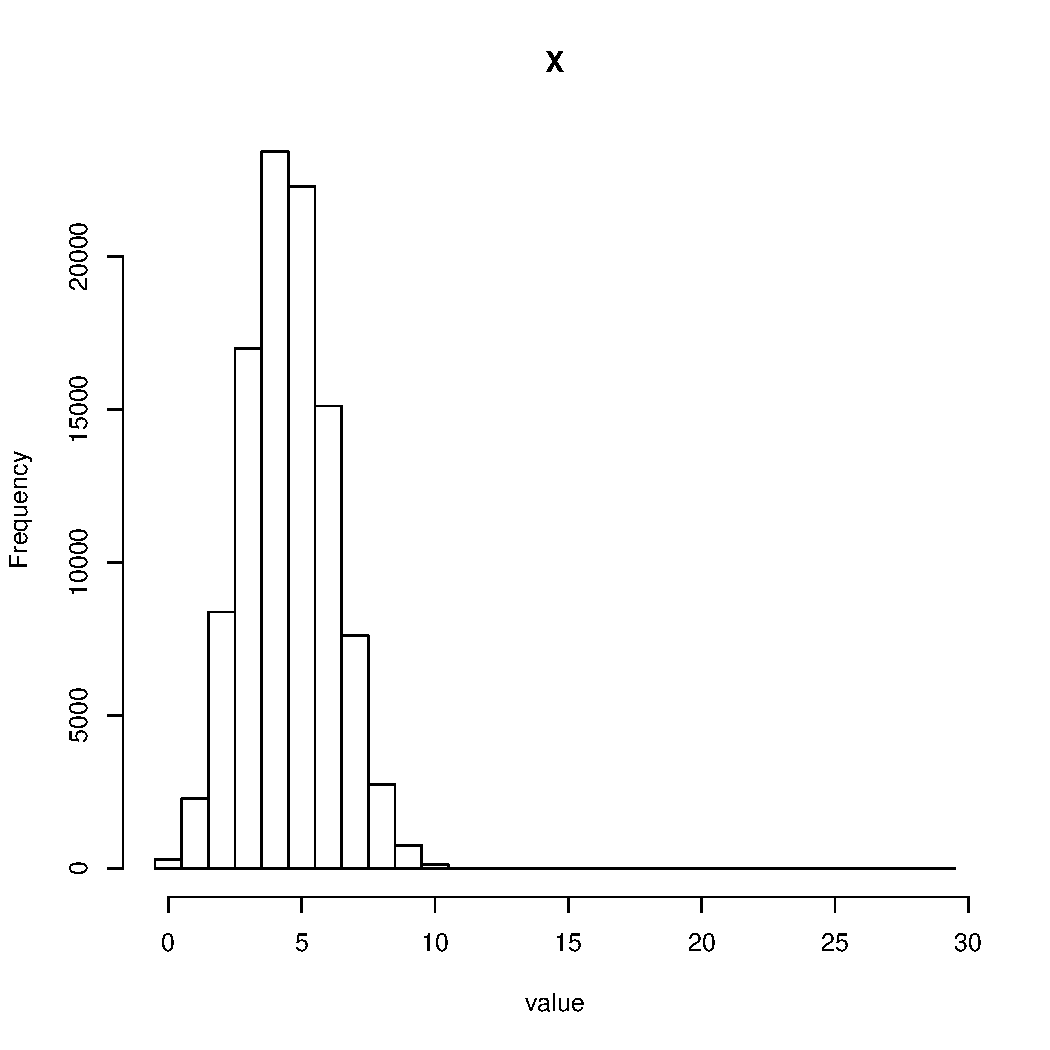
\includegraphics[width=0.5\textwidth]{R/hyper}
  \end{figure}
  How would you estimate the probability of
  observing a value of more 10?\\
  (hint: there is no need to plot the distribution, it is shown as an aid to
  your thinking only)\\
  (4 points)

 
\item You have obtained expression values for 20,000 (i.e. $2 \times 10^4$) genes from two sets of tissue samples
  that were incubated under two different conditions. You have then performed
  a statistical test for differential expression between the two conditions
  for each gene.
  \begin{enumerate}
  \item State your \textit{null}-hypothesis.
  \item What is the probability of observing a p-value less than
    x from a single test if the \textit{null}-hypothesis is true?
  \item What will be the distribution of p-values if the
    \textit{null}-hypothesis is true for all genes?
  \item How many of the 20,000 genes would you expect to have p-values
    less than 0.05 if the \textit{null}-hypothesis is true?
  \item How do you decide what p-value indicates a real effect of
    the condition on gene expression?
  \item How else can you estimate the number of genes whose expression are
    affected by the treatment?
  \end{enumerate}
(10 points)

 

\item What do these equations calculate?

  \begin{minipage}{0.5\textwidth}
    $$ 
    \frac{\sum_{i=1}^{n}{(x_i - \overline{x})^2}}{n-1} 
    $$
  \end{minipage}%
  \begin{minipage}{0.5\textwidth}
    $$
    \frac{\sum_{i=1}^{n}{(x_i - \overline{x})^2}}{n} 
    $$
  \end{minipage}

  Which of them would you normally use and why? Explain the
  relationship between the values obtained from the two equations.\\
  (4 points)


%% \item In the following R-code;
%%    exp.data is a matrix of expression values that 
%%    has been defined previously.
%%    Each column represents a sample 
%%    and each row a gene transcript

%%   \begin{rcode}
  
%%   h.all <- hist( log(exp.data) )
%%   h.sample <- apply( log(exp.data), 2, function(x){ hist(x,
%%     breaks=h.all$breaks) })
  
%%   h.sample.c <- sapply( h.sample, function(x){ x$counts })
%%   \end{rcode}
%%   Describe what is obtained on each line of functional code (1, 2-3, 5).\\
%%   (4 points)

\item The following is part of the help page for the scale function:\\
  \begin{consolecode}
Description:
     scale is generic function whose default method centers and/or
     scales the columns of a numeric matrix.
Usage:    scale(x, center = TRUE, scale = TRUE)
Arguments:
       x: a numeric matrix(like object).
  center: either a logical value or a numeric vector of length equal 
          to the number of columns of x.
   scale: either a logical value or a numeric vector of length equal
          to the number of columns of x.
Details:
     The value of center determines how column centering is
     performed. If center is TRUE then centering is done by 
     subtracting the column means (omitting NA's) of x from 
     their corresponding columns, and if center is FALSE, 
     no centering is done.
     The value of scale determines how column scaling is performed
     (after centering).  If scale is TRUE then scaling is done by 
     dividing the (centered) columns of x by their standard 
     deviations if center is TRUE, and the root mean square otherwise.  
     If scale is FALSE, no scaling is done.

  \end{consolecode}
  
  Given the following R code:\\
  \begin{rcode}
    m <- matrix(1:9, nrow=3)
    ms <- t(scale( t(m), center=TRUE, scale=TRUE ))
  \end{rcode}
  \begin{enumerate}
  \item Draw the matrix m.
  \item Provide an alternate expression that takes m or subsets of m as
    arguments and gives the value of \texttt{ms[3,1]}. You will need to use
    the \texttt{mean()} and \texttt{sd()} functions that give the mean and
    standard deviations for a given vector.
  \item Use \texttt{apply()} to write an expression that converts \texttt{m}
    to \texttt{ms}.
  \end{enumerate}
  (10 points)

\item What's the most important R function?\\
  (1 point)
\end{enumerate}


\end{document}
